\clearpage
\section{Temporal harmonization}
\label{app:temporal}

\subsection{Native clocks and observation boundaries}

Temporal coverage is defined for each sampled implementation and observation type. Its lower boundary may reflect contract deployment, a change in protocol rules, archive availability or the retention limits of a state interface. These boundaries are distinct from the first event found in a table. Table~\ref{tab:temporal_boundaries} summarizes the reasons for the observed scope; Appendix~\ref{app:scope} provides the implementation and source details.

\begingroup
\small\setlength{\tabcolsep}{5pt}\renewcommand{\arraystretch}{1.14}
\begin{longtable}{@{}L{0.13\linewidth} L{0.39\linewidth} L{0.41\linewidth}@{}}
\caption{Native clocks and lower boundaries. First observations do not establish deployment dates.}\label{tab:temporal_boundaries}\\
\toprule Branch & Native clock and observation & Starting boundary and limitation \\
\midrule\endfirsthead
\toprule Branch & Native clock and observation & Starting boundary and limitation \\
\midrule\endhead
UMA & Polygon event blocks; Ethereum DVM blocks. Request-reference timestamps remain separate. & Version-specific registered contracts and scans. The native DVM inputs lack explicit event clocks; only exact retained block matches are recovered. \\
Chainlink & Staking event blocks; ETH/USD \codefield{updated_at} payload and separate execution time. & Staking v0.2 deployment-bound collection; feed history is phase-specific. The native feed table and the common adjacent-window projection have different populations. \\
Tellor & Millisecond report time; aggregate index time; dispute and execution clocks, some with subsecond text. & tellor-1 scan through height 19,890,860. First retained report is at height 317; the later public-opening announcement does not date that event. \\
Flare FTSOv2 & Reward-epoch support, claim execution time and cutoff state remain separate. & Retained reward epochs 228--410; conditions from 251. RewardManager and VoterRegistry have separate deployments. Epoch 411 straddles the cutoff and is outside the closed-epoch panel. \\
Pyth & Solana transaction time; publisher-epoch support; later state snapshot. & Transaction history predates the retained state panel. Its first epoch-end label is later than the beginning of its support interval. The circular buffer does not preserve full deployment history. \\
Chronicle & Ethereum execution block and separate oracle payload time. & Validated historical contract set, scanned from block 0 to the cutoff. The scan boundary and first retained event do not establish deployment. \\
RedStone Push & Ethereum Push execution block and separate payload time. & Pinned Push contracts, scanned from block 0. Pull and AVS activity are outside this observation window. \\
DIA & Lasernet staking event and verified withdrawal execution times. & Deployment-bound staking scan from block 3,874,186. The first withdrawal does not date deployment or the beginning of staking activity. \\
\bottomrule
\end{longtable}
\endgroup


The interpretation of time also depends on the native object. A UMA request-reference timestamp contributes to request identity, whereas the block timestamp dates the recorded event. Tellor report, aggregate and dispute clocks refer to different stages of reporting and adjudication. An epoch or state snapshot represents temporal support or a state observation rather than an instantaneous event.

\subsection{UTC representation and epoch support}

UTC conversion preserves native values, units and precision. Table~\ref{tab:temporal_examples} illustrates second and millisecond clocks, epoch intervals and missing-time handling. Native identifiers and execution order are retained; nanosecond storage does not increase source precision.

Missing EVM times are recovered from consistent same-chain, same-block timestamps, with provenance distinguishing recovered and source-provided clocks. Conflicting or unmatched blocks remain undated.

\begin{table}[!htbp]
\centering\tabstyle
\caption{Native-to-UTC examples from retained observations. Epochs use $[a,b)$ intervals; missing values remain explicit. Record identifiers and source matches accompany the examples.}
\label{tab:temporal_examples}
\begin{tabularx}{\linewidth}{@{}L{.16\linewidth}L{.23\linewidth}L{.25\linewidth}Y@{}}
\toprule\tablehead
Observation & Native value & UTC representation & Interpretation \\
\midrule
\textbf{E1} UMA request & 1667593230 s & 2022-11-04\newline 20:20:30 & Exact second conversion; request-event block time. \\
\textbf{E2} Tellor report & 1746801845665 ms & 2025-05-09\newline 14:44:05.665 & Exact millisecond conversion; fractional seconds retained. \\
\textbf{E3} Pyth epoch & $[1752710400,$\newline $1753315200)$ s & Start: 2025-07-17\newline End: 2025-07-24\newline Both at 00:00:00 & Epoch support interval; no event or payment time inferred. \\
\textbf{E4} Chainlink staking & Missing; Ethereum block 18,671,606 & 2023-11-28\newline 17:27:47 & Recovered from a retained Chronicle record for the same Ethereum block. \\
\textbf{E5} Chainlink staking & Missing; Ethereum block 18,621,068 & Missing & No retained block-time match; value remains missing. \\
\bottomrule
\end{tabularx}
\end{table}


Epoch-based observations are represented by their native start and end boundaries. The retained Flare and Pyth reward intervals have different durations, and neither interval determines when a payment occurred. Figure~\ref{fig:temporal_support} illustrates their alignment near the observation cutoff. A timestamp on a shared epoch boundary belongs to the later interval under the half-open convention. Later state snapshots preserve their own acquisition context and do not establish when historical values became available to participants.

\begin{figure}[!htbp]
\centering
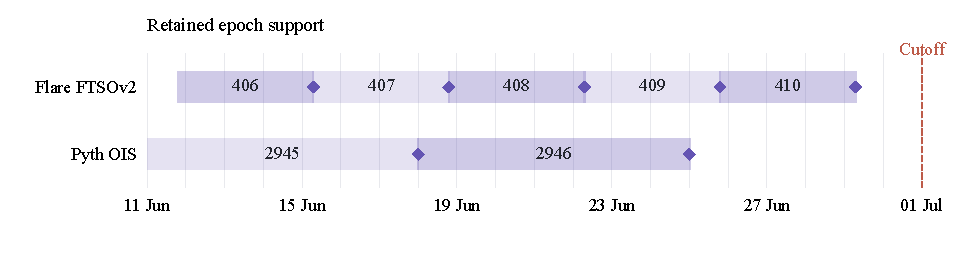
\includegraphics[width=\linewidth]{figures/temporal_epoch_support.pdf}
\caption{Native epochs near the cutoff. Flare and Pyth bars span three and a half and seven days, respectively; diamonds mark epoch-end labels against a daily grid. Labels denote observation intervals, not payments.}
\label{fig:temporal_support}
\end{figure}

\FloatBarrier
\subsection{Temporal availability and coverage}

Timestamp availability is the proportion of retained observations with a valid clock. Historical coverage additionally requires evidence about the period in which a mechanism was active and the intervals successfully collected. A sequence with timestamps on every row can therefore still contain acquisition gaps. Coverage remains unspecified when the underlying observation period cannot be established.

\begin{table}[!htbp]
\centering\tabstyle
\caption{Timestamp availability within retained populations after exact block matching. The Chainlink subset covers staking, withdrawals, reward payments, reward finalization and forfeiture distributions.}
\label{tab:temporal_recovery}
\begin{tabularx}{\linewidth}{@{}Y r Y@{}}
\toprule\tablehead
Observation population & Available & Remaining limitation \\
\midrule
UMA DVM voter accruals & 10.9\% & Execution time is unavailable for unmatched blocks. \\
Chainlink native staking logs & 6.0\% & Retained block references cover only part of the log history. \\
Chainlink analytical subset & 5.0\% & Temporal analysis remains restricted to the dated observations. \\
\bottomrule
\end{tabularx}
\end{table}


Native and UTC timestamps and record selections agree within the tested windows. Subsecond values and native order are preserved, and epoch duration and membership checks support the interval representation. These tests assess processing consistency without establishing clock accuracy or continuous acquisition.


Temporal annotations and the original common representation are separately versioned. Analyses should use a consistent representation and restrict comparisons to compatible observation periods. Daily economic measures further require defined participant roles, assets, economic stages and exposure. Epoch totals should remain attached to their support intervals unless the data justify a more detailed temporal allocation.
